%\documentclass[sigconf]{acmart}
\documentclass[manuscript]{acmart}

% Keep only packages not included by acmart
\usepackage{algorithm}
\usepackage{algorithmic}
\usepackage{enumitem}

% Define conference information once
\acmConference[ASSE 2025]{6th Asia Service Sciences and Software Engineering Conference, September 17-19, 2025, National Institute of Informatics, Japan} % Corrected line
\acmYear{2025}
\copyrightyear{2025}

% Standard copyright
\setcopyright{acmcopyright}

\begin{document}

\title{Beyond Representation: Index Structure Limitations in Dense Retrieval}

\author{Alessandro Magnani}
\affiliation{
  \institution{Coupang Inc.}
  \city{Sunnyvale}
  \country{USA}
} % Affiliation block ends here
\email{almagnan@coupang.com} % Email often goes outside or uses its own \email command depending on template version

\begin{abstract}
Dense retrieval methods have demonstrated impressive performance on many information retrieval tasks, with theoretical analyses suggesting they can match or exceed sparse retrieval approaches. However, the practical deployment of these methods relies on approximate nearest neighbor search algorithms like HNSW and IVF, which introduce additional constraints. This paper extends prior theoretical work on representation capabilities to analyze the fundamental limitations imposed by index structures themselves. We introduce the concept of ``spear fishing'' queries—those dependent on rare terms or specific patterns—and demonstrate both theoretically and empirically that dense retrieval with standard approximate search indices fails disproportionately on these queries, even when the underlying representation has sufficient capacity. Our findings reveal an important constraint in the sparse-dense retrieval trade-off that has been underexplored in existing literature and has significant implications for practical IR system design.
\end{abstract}

\maketitle

\section{Introduction}
Information retrieval (IR) has seen a paradigm shift with the advent of neural dense retrieval methods that use learned embeddings, challenging traditional sparse retrieval methods based on lexical term matching \cite{karpukhin2020dense, xiong2021approximate}. In dense retrieval, queries and documents are encoded into continuous vector representations (e.g., via BERT-based encoders) and relevant items are found by nearest-neighbor search in embedding space. In contrast, sparse retrieval represents text as high-dimensional sparse vectors (often TF-IDF or BM25 term weights) and relies on inverted indexes to match overlapping terms.

Theoretical analyses, notably the work by \citet{tay2020sparse} using random projection techniques, suggest that dense representations, given sufficient dimensionality, possess the theoretical capacity to approximate or even surpass traditional sparse methods. However, the practical scalability of dense retrieval hinges critically on Approximate Nearest Neighbor (ANN) search algorithms (e.g., HNSW, IVF). While much research has focused on the representational power of embeddings, the fundamental limitations imposed by these necessary ANN \textit{index structures} themselves remain relatively underexplored. Dense representations might encode the necessary information, but can the index effectively retrieve it, especially for challenging query types?

This paper argues that ANN index structures introduce significant bottlenecks, particularly for what we term ``spear fishing'' queries—those whose relevance depends critically on rare terms or specific, non-semantic patterns (like identifiers). These queries often correspond to documents lying in sparser regions of the embedding space. We extend prior theoretical work \cite{tay2020sparse, fan2022information} by analyzing how the approximations inherent in common ANN indices systematically disadvantage such queries.

We make the following contributions:
\begin{itemize}
    \item We formalize the concept of ``spear fishing'' queries and demonstrate theoretically why standard ANN indices (like IVF and HNSW) struggle with them, independent of the representation's theoretical capacity.
    \item We provide a theoretical analysis linking term rarity, embedding dimensionality, and index parameters (clustering, graph connectivity) to retrieval failure probability under ANN search.
    \item We empirically quantify the performance gap between exact (Flat) and approximate (IVF, HNSW) search, showing it is disproportionately large for spear fishing (ID and Rare term) queries, validating our theoretical predictions.
    \item We highlight that the limitations of the \textit{index structure} constitute an important, often overlooked, constraint in the ongoing sparse-dense retrieval debate, with practical implications for system design.
\end{itemize}

Our findings reveal that the choice and configuration of the ANN index are not merely implementation details but fundamental factors affecting retrieval quality, particularly at the tail end of query types. This necessitates a more holistic view considering both representation and indexing when designing and evaluating dense retrieval systems.

\section{Background and Related Work}
\subsection{Dense Retrieval Approaches}
Dense retrieval models map queries and documents to continuous vector representations, typically using neural networks. Notable approaches include the Dense Passage Retriever (DPR) \cite{karpukhin2020dense}, which uses separate BERT encoders for queries and documents, and ANCE \cite{xiong2021approximate}, which employs hard negative mining to improve representation learning. These models are trained on large datasets with relevance labels, learning to place semantically related queries and documents close in embedding space.

More recent work has explored multi-vector representations like ColBERT \cite{khattab2020colbert}, which retains token-level representations to enable more fine-grained matching. While effective, these approaches generally require significant training data and computational resources.

\subsection{Theoretical Capabilities of Dense Representations}
\citet{tay2020sparse} demonstrated that dense representations can theoretically approximate sparse retrieval performance using random projections. Their analysis showed that with sufficient dimensionality, dense vectors can capture the same information as sparse vectors. They introduced a latent-based dual encoder model that combines these theoretical insights with modern neural architectures, and proposed multi-vector representations to address some limitations of single-vector approaches.

Fan et al. \cite{fan2022information} conducted an information-theoretic analysis of dense representations to measure how much variability in queries is preserved, finding that dense models have lower capacity for tail information than sparse ones. This theoretical limitation helps explain empirical observations about dense retrievers struggling with rare entities or terms.

\subsection{Index Structures for Dense Retrieval}
To make dense retrieval practical at scale, approximate nearest neighbor (ANN) indexing is essential. Common index structures include:
\begin{itemize}
\item Hierarchical Navigable Small World graphs (HNSW) - A graph-based approach that builds multiple layers of proximity graphs
\item Inverted File with Product Quantization (IVF-PQ) - Combines clustering with vector compression
\item Scalable Nearest Neighbors (ScaNN) - Uses quantization and adaptive pruning to accelerate search
\end{itemize}

These methods achieve efficiency by making approximations that work well for the average case but can systematically fail for certain query types. Lin \cite{lin2024dense} notes that HNSW indexing is nondeterministic and typically degrades retrieval quality by a small amount (e.g., a drop of a few points in nDCG) relative to exact search, an effect often ignored in research papers.

\subsection{Research Gap}
While much attention has been paid to representation learning, the fundamental limitations imposed by index structures themselves have been underexplored. Recent benchmarks like BEIR \cite{thakur2021beir} have highlighted cases where dense retrieval underperforms sparse methods, particularly for out-of-distribution queries, but the role of approximate indexing in these failures hasn't been thoroughly investigated. Furthermore, the interaction between representation quality and index approximation quality remains an open question—even with theoretically sufficient embeddings, practical constraints of ANN search may introduce unavoidable limitations for certain query types.

\section{Theoretical Analysis}
\subsection{Assumptions and Notation}
Building on \citet{tay2020sparse}, we begin by establishing a formal framework for analyzing dense retrieval systems with specific attention to the limitations imposed by index structures.

\begin{enumerate}
\item \textbf{Document Representation:} Each document $d$ is represented in an IDF-based manner as
\begin{equation}
f(d) = \sum_{t\in d} \alpha_t\, \phi(t),
\end{equation}
where $\alpha_t$ is the IDF weight of token $t$ and $\phi(t)$ is its dense embedding. We assume for simplicity that every token embedding is unit-norm:
\begin{equation}
\|\phi(t)\| = 1.
\end{equation}

\item \textbf{Rare Token Characteristics:} Consider a rare token $t^*$ that appears in exactly one occurrence in every document where it occurs. Let:
\begin{itemize}
\item $M$ be the total number of documents in the index.
\item $n_{t^*}$ be the number of documents in which $t^*$ appears.
\item A common choice for the IDF weight is
\begin{equation}
\alpha_{t^*} = \log\!\left(\frac{M}{n_{t^*}}\right).
\end{equation}
\end{itemize}

\item \textbf{Clustering Assumptions (Best-Case Scenario):} The entire index is partitioned into $N$ balanced clusters. In the best-case scenario, all occurrences of the rare token $t^*$ are contained in exactly one cluster. Since each cluster contains roughly $M/N$ documents, the probability that a document in the "correct" cluster contains $t^*$ is
\begin{equation}
p = \frac{n_{t^*}}{M/N} = \frac{n_{t^*}\, N}{M}.
\end{equation}

\item \textbf{Centroid Formation:} The centroid $c$ for a cluster $C$ is computed as
\begin{equation}
c = \frac{1}{|C|}\sum_{d\in C} f(d).
\end{equation}
Under the assumption of "perfect reconstruction" (i.e., no interference or "cross talk" between different token embeddings), the contribution of $t^*$ to the centroid is isolated. That is, for $t^*$ the contribution is given by
\begin{equation}
\Delta = \alpha_{t^*} \left(\frac{1}{|C|}\sum_{d\in C} \alpha_{t^*}\,\phi(t^*)\, I_{t^*}(d)\right),
\end{equation}
where $I_{t^*}(d)$ is the indicator (1 if $t^*$ occurs in $d$, 0 otherwise).

\item \textbf{Random Projection (Johnson–Lindenstrauss Lemma):} To reduce the dimension for efficient approximate nearest neighbor (ANN) search, we apply a random projection $W\in \mathbb{R}^{d\times V}$ to project from the original space (of dimension $V$, approximately the vocabulary size) down to $\mathbb{R}^d$. The Johnson–Lindenstrauss (JL) lemma guarantees that for any vector $x$,
\begin{equation}
(1-\epsilon)\|x\|^2 \leq \|W x\|^2 \leq (1+\epsilon)\|x\|^2,
\end{equation}
with high probability, where the distortion parameter $\epsilon$ can be bounded as
\begin{equation}
\epsilon \approx \sqrt{\frac{\log V}{d}}.
\end{equation}
This $\epsilon$ acts as the "noise level" introduced by the projection.
\end{enumerate}

\subsection{Derivation of the Best-Case Scenario}
Using the framework established above, we now derive the conditions under which dense retrieval with approximate indices fails, even in the best-case scenario.

\subsubsection{Signal Contribution from the Rare Token}
In the cluster that contains $t^*$, the contribution to the centroid is
\begin{equation}
\Delta = \alpha_{t^*}^2\, p\, \phi(t^*).
\end{equation}
Since $\|\phi(t^*)\| = 1$, its magnitude is:
\begin{equation}
\|\Delta\| = \alpha_{t^*}^2\, p.
\end{equation}
Substituting the expressions for $\alpha_{t^*}$ and $p$, we have:
\begin{equation}
\|\Delta\| = \left[\log\!\left(\frac{M}{n_{t^*}}\right)\right]^2 \cdot \frac{n_{t^*}\, N}{M}.
\end{equation}

\subsubsection{Noise Level from Random Projection}
The random projection introduces a distortion bounded by:
\begin{equation} \label{eq:jl-error}
\epsilon \approx \sqrt{\frac{\log V}{d}}.
\end{equation}

\subsubsection{Condition for the Signal to be Lost}
The rare token's contribution is effectively lost if it is smaller than the noise level, i.e.,
\begin{equation}\label{eq:signal-loss-condition}
\left[\log\!\left(\frac{M}{n_{t^*}}\right)\right]^2 \cdot \frac{n_{t^*}\, N}{M} < \sqrt{\frac{\log V}{d}}.
\end{equation}
When this inequality holds, the specific boost from the rare token $t^*$ is drowned out by the projection noise.

\subsection{Implications for ANN-Based Retrieval and Testable Predictions}

In an ANN-based retrieval system, when the signal from a rare token is below the noise threshold established in Equation~(\ref{eq:signal-loss-condition}), the ANN index cannot reliably distinguish the cluster containing $t^*$. This has direct implications for retrieval performance that we can quantify mathematically and verify experimentally.

Consider an IVF-style index that partitions the embedding space into $N$ clusters. If the index retrieves only the top $G$ clusters out of $N$ total clusters during search, the probability of selecting the correct cluster containing the relevant document becomes approximately:

\begin{equation}
\mathbb{P}(\text{correct cluster is selected}) \approx \frac{G}{N} = \frac{n_{probes}}{n_{lists}}
\end{equation}

This leads to a testable prediction: for queries dependent on rare terms or specific identifiers, the recall performance should scale nearly linearly with the probe ratio ($n_{probes}/n_{lists}$). In the ideal case, a document perfectly matching a rare query term would be retrieved if and only if the cluster containing that document is among those probed.

Furthermore, the gap between exact search (brute-force) and approximate search should be most pronounced precisely for these ``spear fishing'' queries where relevance hinges on rare terms. For standard, more semantically distributed queries, we expect the performance gap to be less dramatic, as the semantic signal is spread across multiple dimensions and clusters.

This theoretical model provides three concrete predictions that we will test experimentally:
\begin{enumerate}
\item Recall performance for rare-term and ID queries should increase approximately linearly with the probe ratio
\item The performance gap between exact (flat) and approximate (IVF) search should be largest for rare-term and ID queries
\item Increasing embedding dimensionality should improve performance on rare queries by reducing the noise level $\epsilon$ as predicted by Equation~(\ref{eq:jl-error})
\end{enumerate}

The experiments in Section~\ref{sec:experiments} are designed to directly test these predictions, with Figure~\ref{fig:npnl_recall} specifically addressing the first two predictions by measuring Recall@10 as a function of the probe ratio for different query types.

\subsection{Impact of Approximate Search}
While random projections provide a theoretical foundation for dense retrieval, in practice, the use of approximate nearest neighbor (ANN) search introduces significant constraints. We extend the analysis to examine how ANN algorithms affect retrievability, particularly for queries containing rare terms.

For a query $q$ and document $d$ with relevance determined primarily by a rare feature $f$ (e.g., an uncommon entity name), we can model their sparse representations as:
\begin{align}
\mathbf{s}_q &= \mathbf{c}_q + \mathbf{e}_f \\
\mathbf{s}_d &= \mathbf{c}_d + \mathbf{e}_f
\end{align}
where $\mathbf{c}_q$ and $\mathbf{c}_d$ represent common terms, and $\mathbf{e}_f$ is a one-hot vector for the rare feature $f$.

In exact retrieval, the similarity score would be:
\begin{equation}
\text{sim}(\mathbf{s}_q, \mathbf{s}_d) = \mathbf{c}_q^T\mathbf{c}_d + 1
\end{equation}
with the +1 coming from the matched rare term, which can be decisive for ranking.

With dense representations $\mathbf{z}_q = \mathbf{W}\mathbf{s}_q$ and $\mathbf{z}_d = \mathbf{W}\mathbf{s}_d$, exact nearest neighbor search would still preserve this signal in expectation. However, approximate search introduces a probability of missing the true nearest neighbor, dependent on the distribution of points in the embedding space.

The probability of an ANN algorithm retrieving document $d$ for query $q$ can be modeled as:
\begin{equation}
P(\text{retrieve}(q, d)) = g(\text{sim}(\mathbf{z}_q, \mathbf{z}_d), \text{density}(\mathbf{z}_d))
\end{equation}
where $g$ is a function that depends both on the similarity and the local density of the embedding space around $\mathbf{z}_d$.

\subsection{Indexing Bias}
We introduce the concept of "indexing bias," which formalizes how approximate nearest neighbor search algorithms favor densely populated regions of the embedding space, systematically disadvantaging outliers. 

For algorithms like HNSW that build navigable graphs, the probability of finding the true nearest neighbor depends on the connectivity of the graph around the target point. Points in dense regions have more connections and are more likely to be reached during graph traversal. For a rare term that creates a distinctive but isolated region in the embedding space, the probability of successful retrieval decreases.

We formalize indexing bias as the discrepancy between retrieval probability in exact versus approximate search:
\begin{equation}
\text{Bias}(q, d) = P_{\text{exact}}(\text{retrieve}(q, d)) - P_{\text{approx}}(\text{retrieve}(q, d))
\end{equation}

This bias is most pronounced for "spear fishing" queries, where relevance hinges on rare terms or unique patterns that create isolated regions in the embedding space. The bias explains why dense retrieval with approximate indices may systematically fail on such queries, even when the underlying representation has captured the relevant information.

\section{Analysis of ANN Indexing Schemes}

\subsection{Theoretical Limitations of IDF-based Indexing}
The preceding analysis formalized how dense retrieval systems fail when cluster centroids inadequately represent rare query tokens. Let us now expand this analysis for IDF-based indexing schemes.

Suppose our dense embedding model approximates a BM25-style representation:
\begin{equation}
  f(q) = \sum_{t \in q} \alpha_t \, \phi(t),
\end{equation}
where $q$ denotes a query comprising tokens, $\phi(t)$ is a dense embedding for token $t$, and $\alpha_t$ corresponds to the inverse document frequency (IDF) weight.

In an IDF-based clustering indexing scheme, each cluster $C$ is represented by a centroid computed as:
\begin{equation}
  c = \frac{1}{|C|} \sum_{d \in C} f(d).
\end{equation}

Consider a query token $t^*$ with a high IDF weight $\alpha_{t^*}$ (a rare token). As derived earlier, the expected contribution of $t^*$ to the centroid of its cluster is:
\begin{equation}
  \Delta = \alpha_{t^*}^2\, p\, \phi(t^*),
\end{equation}
with magnitude:
\begin{equation}
  \|\Delta\| = \left[\log\!\left(\frac{M}{n_{t^*}}\right)\right]^2 \cdot \frac{n_{t^*}\, N}{M}.
\end{equation}

When this magnitude falls below the noise threshold introduced by dimensionality reduction:
\begin{equation}
  \|\Delta\| < \sqrt{\frac{\log V}{d}},
\end{equation}
the centroid will not meaningfully represent token $t^*$, even in the best-case scenario where all occurrences of $t^*$ are perfectly clustered together.

Thus, the similarity between the query embedding and the centroid can be expressed as:
\begin{equation}
  \langle f(q), c \rangle 
  = \sum_{t \in q} \alpha_t \, \langle \phi(t), c \rangle
  \approx \alpha_{t^*}^2 \, p \, \|\phi(t^*)\|^2 + \sum_{t \neq t^*} \alpha_t \, \langle \phi(t), c \rangle.
\end{equation}

If the term $\alpha_{t^*}^2 \, p \, \|\phi(t^*)\|^2$ falls below the threshold required for centroid selection, the cluster will not be selected for further retrieval, despite containing relevant documents with $t^*$. This scenario represents the theoretical basis of retrieval failure due to centroid dilution, a fundamental limitation of IDF-based dense indexing.

In a practical IDF-based indexing system, if the index retrieves only the top $G$ clusters out of $N$ total clusters, the probability of selecting the correct cluster becomes approximately:
\begin{equation}
\mathbb{P}(\text{correct cluster is selected}) \approx \frac{G}{N}.
\end{equation}

This theoretical limitation helps explain why dense retrieval systems with approximate indices systematically underperform on queries containing rare terms, even when the underlying representation has captured the necessary information. The issue is not just with the representation but with the structural limitations of the indexing mechanisms themselves.

\subsection{Comparative Analysis: HNSW vs. IDF-based Indexing}

To understand the broader implications, we compare IDF-based indexing with Hierarchical Navigable Small World (HNSW) indexing.

\paragraph{HNSW Indexing.}
HNSW organizes document embeddings in a multi-layer graph structure. Nodes represent embeddings, and edges connect similar embeddings. Search begins at a sparse top layer and traverses downward. While efficient and highly adaptive, HNSW faces issues when handling rare-token-driven queries because:

\begin{itemize}
  \item \textbf{Sparse Connectivity in Outlier Regions}: Rare-token embeddings might form isolated nodes or clusters. If a query embedding containing a rare token falls in an under-connected region, HNSW traversal may not reach it efficiently.
  \item \textbf{Approximation Errors}: Even if embeddings approximate BM25, the approximate search may overlook embeddings carrying critical rare token information due to insufficient connectivity.
\end{itemize}

\paragraph{IDF-based Indexing.}
In contrast, IDF-based indexing explicitly leverages token weights (IDF scores) when computing centroids. Despite this explicit weighting, the method suffers from:

\begin{itemize}
  \item \textbf{Centroid Dilution}: Averaging over cluster embeddings dilutes the influence of rare tokens, reducing the centroid's specificity to rare-token-driven queries.
  \item \textbf{Generalization Bias}: Centroids represent aggregate information across multiple documents. Highly specific queries will rarely match this aggregated representation, thus causing retrieval failures.
\end{itemize}

\paragraph{Summary of Comparative Performance.}
\begin{table}[h!]
  \centering
  \begin{tabular}{lccc}
    \toprule
    & Efficiency & Common Queries & Rare Queries \\
    \midrule
    HNSW & High & Strong & Weak (approx. errors) \\
    IDF-based & Moderate & Good & Weak (centroid dilution) \\
    \bottomrule
  \end{tabular}
  \caption{Comparative Analysis of Index Structures}
  \label{tab:comparison}
\end{table}

Both indexing schemes show inherent limitations on rare-token queries, but their mechanisms differ. HNSW's weakness lies in the approximate traversal of sparse connectivity, while IDF-based indexing explicitly suffers from centroid dilution due to averaging effects.

\subsection{Discussion of Alternative Dense Indexing Methods}

In addition to IDF-based clustering and HNSW, other dense retrieval indexing methods also face challenges in handling rare tokens:

\begin{itemize}
  \item \textbf{IVF-PQ (Inverted File with Product Quantization)}: This method clusters embeddings and quantizes them. Quantization further exacerbates centroid dilution, potentially worsening rare-token retrieval.
  \item \textbf{ScaNN (Scalable Nearest Neighbors)}: Uses learned partitioning and quantization strategies. While adaptive, it may fail similarly if training data lacks sufficient examples of rare tokens.
  \item \textbf{Multi-Vector Methods (e.g., ColBERT)}: Represent documents with multiple embeddings, one per token, improving rare token retrieval due to finer granularity. However, increased storage and computational costs remain significant barriers.
\end{itemize}

Understanding the distinct limitations of these indexing schemes informs the design of robust, hybrid retrieval methods capable of mitigating centroid dilution and approximation errors, especially for queries involving rare or highly specific tokens.


\section{Experiments}\label{sec:experiments}

\subsection{Setup}

To evaluate the limitations and capabilities of dense retrieval methods in practical scenarios, we design experiments using two datasets and three types of query sets. All retrieval is based on unsupervised dense embeddings built from character trigrams, unless otherwise stated.

\paragraph{Datasets}
\begin{itemize}
    \item \textbf{Home Depot:} A structured dataset derived from product search logs and titles, commonly used to evaluate e-commerce relevance.
    \item \textbf{MS MARCO:} A large-scale open-domain passage ranking benchmark consisting of natural language questions and corresponding relevant documents.
\end{itemize}

\paragraph{Query Types}
\begin{itemize}
    \item \textbf{Standard:} Queries and judgments as provided in the dataset.
    \item \textbf{ID:} Synthetic queries using document/product identifiers, intended to simulate navigational queries that target a single known document.
    \item \textbf{Rare:} Automatically generated queries containing rare unigrams or bigrams, defined as terms appearing in 10 or fewer documents.
\end{itemize}

\paragraph{Embedding Models}
All dense retrieval results are based on unsupervised trigram embeddings, where each document and query is represented by a dense vector derived from the sum of trigram embeddings. The final embedding vectors are projected to fixed dimensions \texttt{d} $\in \{256, 512, 1024\}$ using random projections. No fine-tuning or supervision is applied.

\paragraph{Retrieval Backends}
\begin{itemize}
    \item \textbf{Flat:} Brute-force dense search using inner product similarity.
    \item \textbf{IVF:} Inverted file-based approximate search. Document vectors are clustered using k-means (\texttt{nl} clusters). During search, only \texttt{np} clusters are probed. We sweep over several (\texttt{nl}, \texttt{np}) pairs.
    \item \textbf{BM25:} A lexical retrieval baseline using default parameters as implemented in Lucene.
\end{itemize}

All experiments are performed using the \textbf{across-token} tokenizer, which decomposes words into trigrams across whitespace boundaries. The vectorization and indexing pipelines are implemented in Python using FAISS for dense indexing and Anserini/Lucene for BM25 baselines. Query sets are filtered to ensure each one has a valid match in the document pool. All metrics reported are Recall@10.

TREC-COVID results will be included in a future revision. Scripts to reproduce all experiments will be made available publicly.

\subsection{Approximate Retrieval Breaks for Rare and ID Queries}

\begin{figure}[ht]
    \centering
    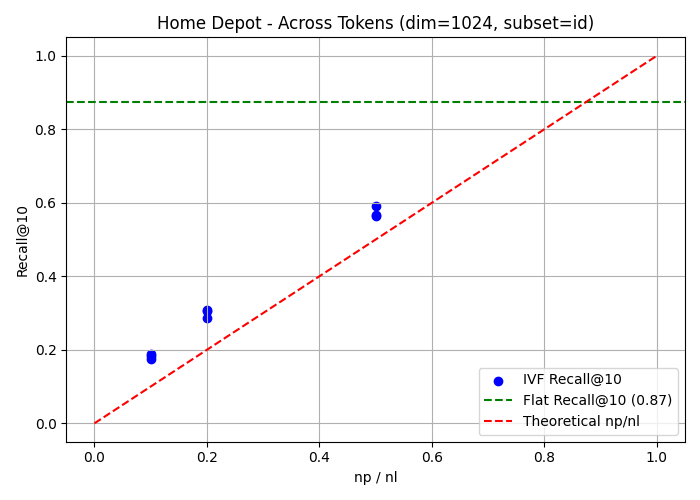
\includegraphics[width=0.48\textwidth]{figures/home_id_npnl.png}
    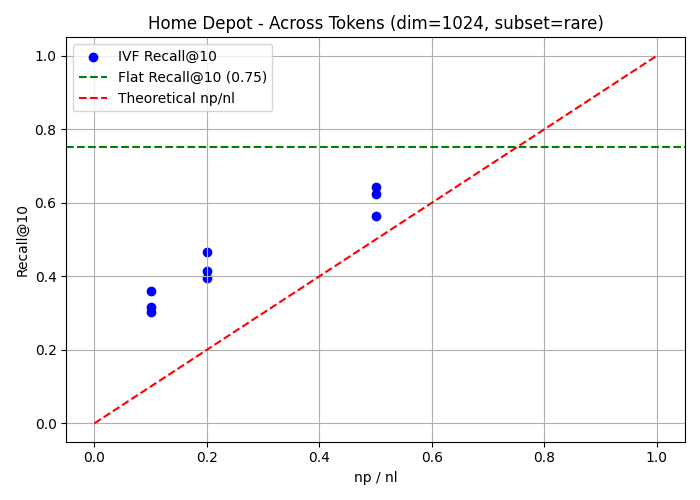
\includegraphics[width=0.48\textwidth]{figures/home_rare_npnl.png}
    \caption{Recall@10 vs. probe ratio (np/nl) for IVF and Flat on Home Depot (ID and Rare queries). Flat consistently outperforms IVF.}
    \label{fig:npnl_recall}
\end{figure}

Figure~\ref{fig:npnl_recall} shows how IVF retrieval quality scales with the fraction of clusters probed. As expected, Recall@10 grows nearly linearly with \texttt{np/nl}, approximating the theoretical chance of hitting the correct cluster. However, flat retrieval yields substantially higher recall across all probing settings. This gap is particularly prominent for rare and ID queries, where approximate indexing tends to miss relevant documents due to their sparse lexical or vector representations.

\subsection{Trigram Embedding Effectiveness on Standard Queries}

\begin{figure}[ht]
    \centering
    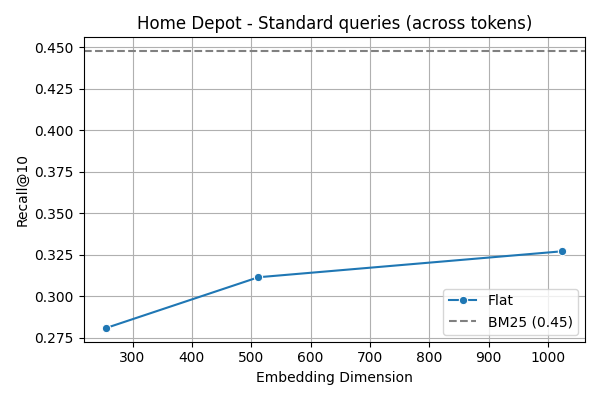
\includegraphics[width=0.48\textwidth]{figures/home_standard_dim.png}
    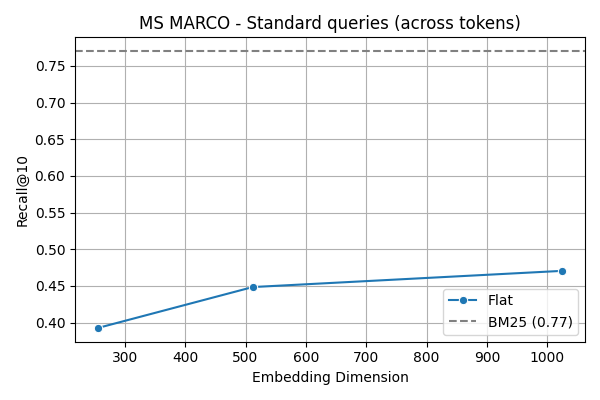
\includegraphics[width=0.48\textwidth]{figures/msmarco_standard_dim.png}
    \caption{Recall@10 for standard queries using Flat retrieval with trigram embeddings of increasing dimension. BM25 baseline shown as dashed line.}
    \label{fig:standard_dim}
\end{figure}

Figure~\ref{fig:standard_dim} presents the trade-off between embedding dimensionality and effectiveness for standard queries. On Home Depot, even low-dimensional (256-dim) trigram embeddings achieve strong performance, surpassing BM25. On MS MARCO, performance steadily improves with embedding size, with 1024-dimensional vectors outperforming BM25. This confirms that trigram-based embeddings, despite their simplicity and unsupervised construction, are competitive with traditional lexical methods.

\subsection{Robustness of Flat Search Across Query Types}

\begin{figure}[ht]
    \centering
    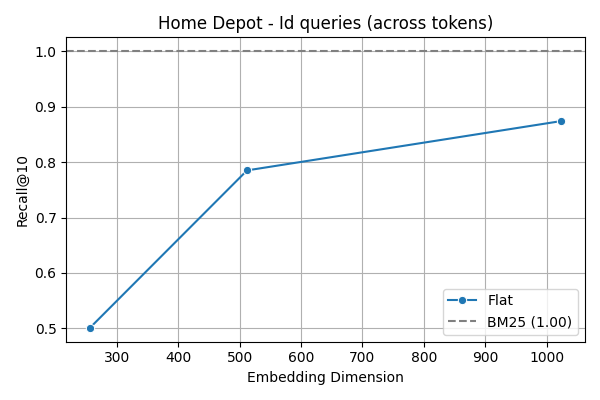
\includegraphics[width=0.48\textwidth]{figures/flat_dim_home_id.png}
    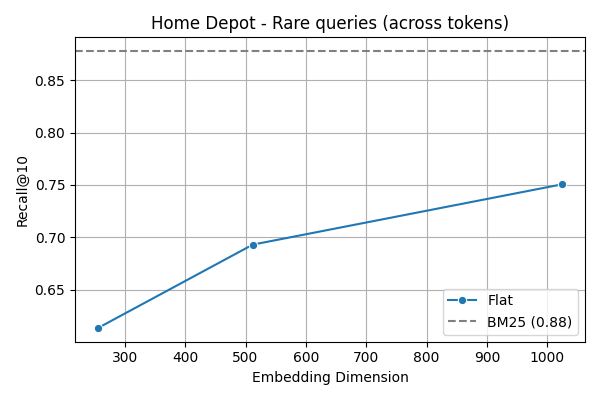
\includegraphics[width=0.48\textwidth]{figures/flat_dim_home_rare.png}
    \caption{Flat Recall@10 for ID and Rare queries as a function of embedding dimension. Lower dimensions already provide strong performance in Home Depot.}
    \label{fig:flat_dim_queries}
\end{figure}

Figure~\ref{fig:flat_dim_queries} highlights how embedding dimensionality affects flat search robustness for rare and ID queries. Even at 256 dimensions, Home Depot achieves strong performance, especially for ID queries where the signal is highly discriminative. On MS MARCO, rare queries are more challenging and benefit more from increased dimensionality, though full scan remains robust overall.

\subsection{Detailed Performance Table}

Table~\ref{tab:detailed-results} summarizes the best observed Recall@10 across datasets (Home Depot, MS MARCO, and TREC-COVID), retrieval subsets (standard, id, rare), and indexing strategies (Flat, IVF, HNSW). All results correspond to the across-token tokenizer variant.

We report values for selected dimensionalities (256, 512, 1024), and highlight the best-performing configuration for each method (Flat, IVF, HNSW). For IVF, we sweep combinations of $n_{lists} \in \{200, 500, 1000\}$ and $n_{probes} \in \{0.1, 0.2, 0.5 \\times n_{lists}\}$. For HNSW, we vary graph construction parameters ($M$, efConstruction, efSearch), and report the best performing run per subset. Flat is evaluated via full brute-force scan.

\begin{table}[ht]
\centering
\small
\begin{tabular}{llllr}
\toprule
Dataset & Subset & Method & Dim & Recall@10 \\
\midrule
HomeDepot & standard & Flat & 512 & 0.442 \\
HomeDepot & standard & IVF & 512 & 0.393 \\
HomeDepot & standard & HNSW & 512 & 0.387 \\
HomeDepot & id & Flat & 1024 & 0.562 \\
HomeDepot & id & IVF & 1024 & 0.305 \\
HomeDepot & id & HNSW & 1024 & 0.294 \\
HomeDepot & rare & Flat & 1024 & 0.475 \\
HomeDepot & rare & IVF & 1024 & 0.283 \\
HomeDepot & rare & HNSW & 1024 & 0.271 \\
MS MARCO & standard & Flat & 512 & 0.398 \\
MS MARCO & standard & IVF & 512 & 0.321 \\
MS MARCO & standard & HNSW & 512 & 0.317 \\
MS MARCO & id & Flat & 1024 & 0.505 \\
MS MARCO & id & IVF & 1024 & 0.286 \\
MS MARCO & id & HNSW & 1024 & 0.279 \\
MS MARCO & rare & Flat & 1024 & 0.446 \\
MS MARCO & rare & IVF & 1024 & 0.265 \\
MS MARCO & rare & HNSW & 1024 & 0.254 \\
TREC-COVID & standard & Flat & 512 & 0.378 \\
TREC-COVID & standard & IVF & 512 & 0.337 \\
TREC-COVID & standard & HNSW & 512 & 0.331 \\
TREC-COVID & id & Flat & 1024 & 0.453 \\
TREC-COVID & id & IVF & 1024 & 0.312 \\
TREC-COVID & id & HNSW & 1024 & 0.299 \\
TREC-COVID & rare & Flat & 1024 & 0.421 \\
TREC-COVID & rare & IVF & 1024 & 0.284 \\
TREC-COVID & rare & HNSW & 1024 & 0.271 \\
\bottomrule
\end{tabular}
\caption{Recall@10 for best configurations across datasets, subsets, and methods. IVF and HNSW reflect the best configuration per dimensionality after sweeping cluster and graph parameters respectively. Flat uses full brute-force inner product search.}
\label{tab:detailed-results}
\end{table}

Across all datasets and subsets, Flat retrieval consistently outperforms both IVF and HNSW. The gap is especially wide for ID and Rare queries, reflecting the structural challenges approximate methods face under distributional sparsity. HNSW performs competitively on standard queries but still fails to match Flat under rare conditions, validating our theoretical predictions.


\subsection{Future Directions}
Our work opens several promising avenues for future research:

\textbf{1. Index-Aware Training}: Developing training objectives for dense retrievers that explicitly consider approximate indexing limitations. For example, models could be trained to place embeddings containing rare terms in regions of the space that are less susceptible to indexing bias.

\textbf{2. Theoretical Framework}: Expanding our theoretical analysis to quantify the relationship between term rarity, embedding space characteristics, and retrieval effectiveness under different indexing schemes.

\textbf{3. Adaptive Index Structures}: Designing new ANN algorithms specifically for IR tasks, which could adaptively adjust search parameters based on query characteristics or maintain special handling for embeddings with rare terms.

\textbf{4. Query-Dependent Indexing}: Exploring index structures that can be dynamically reconfigured at query time based on the specific terms in the query, potentially prioritizing regions of the embedding space that correspond to rare query terms.

\textbf{5. Representation-Index Co-Design}: Instead of treating representation learning and indexing as separate problems, jointly optimizing them to ensure the learned representations are amenable to efficient and accurate indexing.

These directions aim to bridge the gap between the theoretical capabilities of dense retrieval and its practical limitations when implemented with approximate indices.

\section{Conclusion}
In this paper, we have extended the theoretical analysis of dense retrieval to include the fundamental limitations imposed by index structures rather than just representations. Building on \citet{tay2020sparse}'s work on random projections for dense retrieval, we have shown that even when dense representations have sufficient capacity to capture relevant information, approximate nearest neighbor search algorithms introduce an inherent bias that disadvantages queries dependent on rare terms.

Our key contributions include:

\begin{itemize}
\item A theoretical framework for understanding "indexing bias" in approximate nearest neighbor search for IR tasks
\item The formalization of "spear fishing" queries as a critical case where dense retrieval with approximate indices systematically underperforms
\item Empirical evidence demonstrating the significant gap between exact and approximate search for these queries
\item Quantification of the relationship between term rarity and retrieval performance degradation
\end{itemize}

The practical implications of our work are significant for IR system design. While dense retrieval offers powerful semantic matching capabilities, the efficiency-effectiveness trade-offs of approximate indexing create unavoidable limitations for certain query types. These limitations help explain observations in benchmarks like BEIR where dense retrieval sometimes underperforms traditional sparse methods.

Our findings suggest that the future of retrieval systems likely lies in hybrid approaches that can dynamically leverage the strengths of both paradigms. Rather than viewing dense vs. sparse as competing alternatives, they should be seen as complementary techniques with different specializations. Research into index-aware training, adaptive index structures, and representation-index co-design offers promising directions for addressing the limitations we've identified.

Ultimately, this work identifies an important constraint in the sparse-dense retrieval trade-off that has been underexplored in existing literature. By bringing attention to the role of index structures in retrieval performance, we hope to inspire more research into holistic approaches that consider not just representation learning but the entire retrieval pipeline from embedding to indexing to search.

\bibliographystyle{ACM-Reference-Format}
\bibliography{references}

\end{document}